\documentclass[tikz,border=7pt]{standalone}
\usepackage{amsmath}
\usetikzlibrary{arrows.meta,positioning,fit}

\tikzset{
  box/.style={draw,rectangle,minimum width=38mm,minimum height=18mm,align=center},
  port/.style={draw,circle,minimum size=5mm,inner sep=0pt},
  arr/.style={-{Latex[length=2mm]},thick}
}

\begin{document}
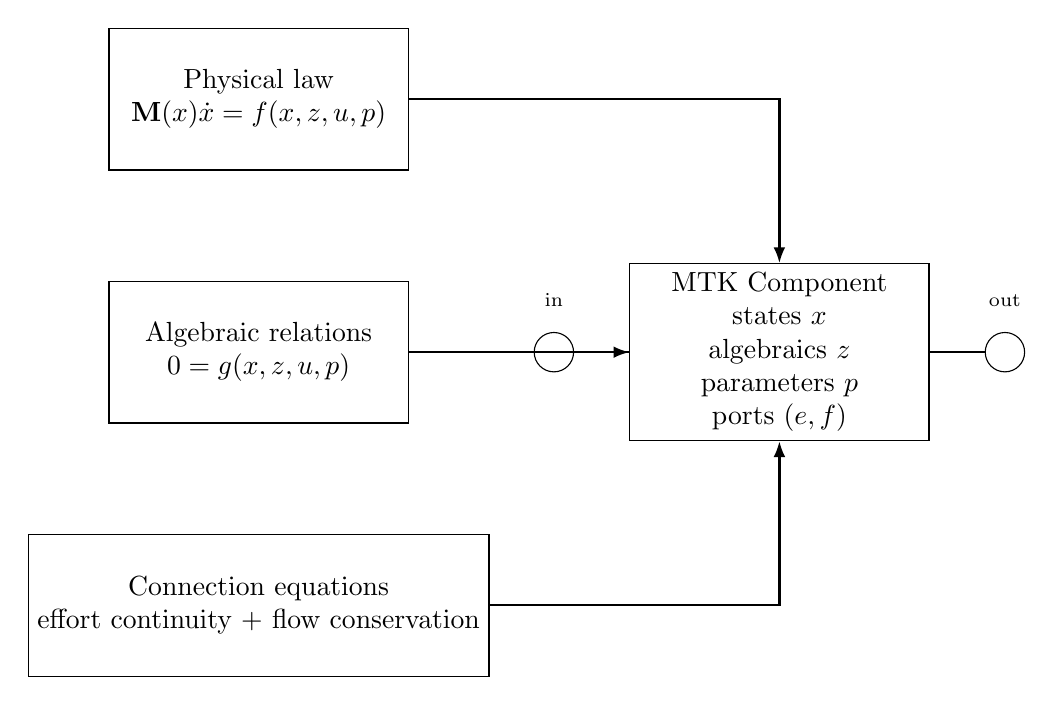
\begin{tikzpicture}[node distance=14mm and 16mm]

\node[box] (physics) {
Physical law\\
$\mathbf{M}(x)\dot x=f(x,z,u,p)$
};

\node[box,below=of physics] (alg) {
Algebraic relations\\
$0=g(x,z,u,p)$
};

\node[box,below=of alg] (conn) {
Connection equations\\
effort continuity + flow conservation
};

\node[box,right=28mm of alg] (component) {
MTK Component\\
states $x$\\
algebraics $z$\\
parameters $p$\\
ports $(e,f)$
};

\node[port,left=7mm of component] (pin) {};
\node[port,right=7mm of component] (pout) {};

\draw[arr] (physics.east) -| (component.north);
\draw[arr] (alg.east) -- (component.west);
\draw[arr] (conn.east) -| (component.south);

\draw[thick] (pin) -- (component.west);
\draw[thick] (component.east) -- (pout);

\node[above=2mm of pin] {\scriptsize in};
\node[above=2mm of pout] {\scriptsize out};

\end{tikzpicture}
\end{document}
